\newpage
\chapter{METODE PENELITIAN} \label{Bab III}

\section{Alur Penelitian} \label{III.Alur}
Penelitian ini merancang dan mengevaluasi sistem QA PDF berbahasa Indonesia berbasis
\textit{transformer} dengan \textit{fine-tuning} IndoBERT-Lite pada IndoQA
\cite{wilie2020indobert,indoqa2023}. Kerangka kerja mengikuti tahapan:
\begin{enumerate}[noitemsep]
    \item Akuisisi dan kurasi data (IndoQA + PDF institusional).
    \item Ekstraksi \& segmentasi PDF (layout-aware dan \textit{fixed window}).
    \item Indeks \& \textit{retrieval} (BM25 baseline; opsional dense).
    \item \textit{Reader} ekstraktif (IndoBERT-Lite di-\textit{fine-tune}).
    \item Evaluasi berlapis (komponen, end-to-end, ablation, V\&V).
\end{enumerate}

Visual alur penelitian ditunjukkan pada Gambar \ref{fig:alur-penelitian}.

\begin{figure}[H]
    \centering
    \usetikzlibrary{arrows.meta, positioning, shapes.geometric}
    \resizebox{0.9\linewidth}{!}{%
        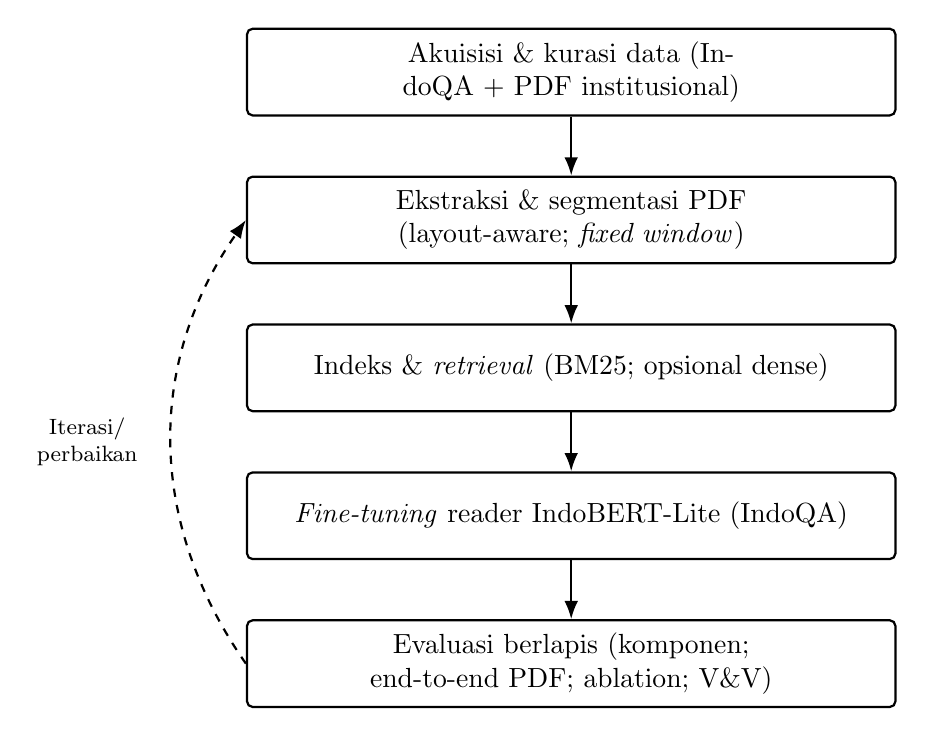
\begin{tikzpicture}[
            node distance=0.75cm,
            >=Latex,
            process/.style={rectangle, rounded corners=2pt, draw=black, thick, text width=8cm, minimum height=1.1cm, align=center},
            feedback/.style={->, thick, dashed}
        ]
            \node (data) [process] {Akuisisi \& kurasi data (IndoQA + PDF institusional)};
            \node (extract) [process, below=of data] {Ekstraksi \& segmentasi PDF (layout-aware; \textit{fixed window})};
            \node (index) [process, below=of extract] {Indeks \& \textit{retrieval} (BM25; opsional dense)};
            \node (reader) [process, below=of index] {\textit{Fine-tuning} reader IndoBERT-Lite (IndoQA)};
            \node (eval) [process, below=of reader] {Evaluasi berlapis (komponen; end-to-end PDF; ablation; V\&V)};

            \draw[->, thick] (data) -- (extract);
            \draw[->, thick] (extract) -- (index);
            \draw[->, thick] (index) -- (reader);
            \draw[->, thick] (reader) -- (eval);
            \draw[feedback] (eval.west) to[bend left=35] node[left=0.3cm, align=center, font=\footnotesize]{Iterasi/\\perbaikan} (extract.west);
        \end{tikzpicture}%
    }
    \caption{Alur penelitian sistem QA PDF berbasis IndoBERT-Lite.}
    \label{fig:alur-penelitian}
\end{figure}

\section{Metode Pengumpulan Data} \label{III.Pengumpulan}
Sumber data sekunder. Dataset IndoQA \cite{indoqa2023} (konteks--pertanyaan--
jawaban) digunakan untuk \textit{fine-tuning} dan validasi reader, dengan split
train/val/test (80/10/10 atau sesuai kartu dataset).

Sumber data dari file atau dokumen berupa PDF. Dipilih 1--2 PDF institusional (SOP/peraturan)
berteks (non-scan), tebal $\geq$30 halaman, terstruktur (bab/subbab). Ekstraksi teks
memakai \texttt{pdfminer.six}/\texttt{PyPDF2}; OCR dikecualikan sesuai batasan.

Gold standard PDF. Disusun 100--200 pasang Q--A dari PDF oleh dua anotator;
kesepakatan dihitung dengan Cohen’s $\kappa$ (target $\geq$ 0{,}75). Pertanyaan disusun
berdasar kebutuhan domain; data sensitif dihapus, memakai dokumen publik/izin internal
dan atribusi sumber.

\section{Metode Perancangan/Pengembangan} \label{III.Pengembangan}
\subsection{Arsitektur Sistem}
Modular: ingestion PDF $\rightarrow$ segmentasi $\rightarrow$ indeks $\rightarrow$
retrieval $\rightarrow$ reader (QA) $\rightarrow$ pelacakan sumber $\rightarrow$
antarmuka. Konsep \textit{retrieval-augmented} \cite{lewis2020rag,karpukhin2020dpr} dan
\textit{transformer} \cite{vaswani2017attention,devlin2019bert,wilie2020indobert} menjadi
dasar, sementara PDFTriage menekankan struktur dokumen \cite{saad2023pdftriage}.

\subsection{Pra-pemrosesan dan Segmentasi}
Tahap ini menormalkan teks PDF yang sering berisi spasi/kode rusak dan batas paragraf
tak konsisten, agar kandidat paragraf stabil untuk \textit{retrieval} dan reader.
\begin{itemize}
    \item Normalisasi karakter (Unicode, spasi), penggabungan tanda baca per kalimat/
    paragraf. Untuk retrieval sparse: \textit{lowercase}, normalisasi angka/tanggal,
    \textit{stopword} opsional; untuk reader: teks dipertahankan apa adanya.
    \item Segmentasi layout-aware: deteksi heading/subheading, pecah per subbagian atau
    paragraf logis (150--250 kata). Fallback: jendela 384 token dengan \textit{stride}
    128. Struktur membantu keterlacakan sumber \cite{saad2023pdftriage}.
\end{itemize}

\subsection{Indeks dan Retrieval}
Retrieval sparse (BM25) dipakai sebagai baseline yang stabil untuk dokumen panjang,
sedangkan dense retrieval hanya pembanding recall; \textit{top-k} menjaga beban reader.
\begin{itemize}
    \item BM25 (Pyserini/Lucene) sebagai baseline: $k1\approx0{,}9$--$1{,}2$, $b\approx
    0{,}4$--$0{,}75$, \textit{top-k} awal = 10.
    \item Opsional dense retrieval (mis. bi-encoder SEA-LION) untuk studi banding
    Recall@k.
    \item \textit{Top-k} (5--10) paragraf kandidat dikirim ke reader.
\end{itemize}

\subsection{Model QA dan Fine-tuning}
IndoBERT-Lite dipilih karena ringan namun terlatih SQuAD-ID; \textit{fine-tuning} pada
IndoQA memindahkan pengetahuan ke domain PDF. Hiperparameter mengikuti praktik standar
QA ekstraktif agar konvergen dengan sumber daya terbatas.
\begin{itemize}
    \item Basis: \texttt{Wikidepia/indobert-lite-squad} (extractive QA).
    \item Data: IndoQA train/val/test.
    \item Hiperparameter awal: \texttt{max\_seq\_length}=384, \texttt{doc\_stride}=128,
    \texttt{max\_answer\_length}=30, \texttt{batch\_size}=16, \texttt{lr}=2e-5,
    \texttt{epochs}=3--5, \texttt{weight\_decay}=0.01, \texttt{warmup\_ratio}=0.1, fp16,
    \texttt{seed}=42, \textit{early stopping} berdasar F1 (patience 2).
\end{itemize}

\subsection{Inferensi End-to-End}
Pipeline mengalir dari pertanyaan ke retrieval kandidat lalu reader memilih span
terbaik; skor membantu memilih jawaban dan melampirkan sumber halaman/paragraf.
Menerima pertanyaan $\rightarrow$ \textit{retrieve} \textit{top-k} paragraf $\rightarrow$
reader memproduksi span jawaban + skor $\rightarrow$ pilih skor tertinggi $\rightarrow$
kembalikan jawaban beserta paragraf/halaman sumber.

\subsection{Kontrol Versi \& Reproduksibilitas}
Reproducibility dijaga lewat berkas lingkungan, konfigurasi eksperimen, dan jejak
versi sehingga eksperimen dapat diulang, diaudit, atau dilanjutkan.
\begin{itemize}
    \item Berkas lingkungan (\texttt{requirements.txt}), konfigurasi YAML untuk
    hiperparameter, \textit{random seed}, dan jejak \textit{commit} model.
    \item \textit{Experiment tracking} (MLflow/Weights \& Biases) untuk metrik.
\end{itemize}

\section{Metode Pengujian/Validasi} \label{III.Pengujian}
\subsection{Evaluasi Komponen}
Metrik dipilih untuk memisahkan kinerja retrieval dan reader, sehingga sumber galat
terlihat jelas sebelum diuji end-to-end.
\begin{itemize}
    \item Retrieval-only: Recall@k (k $\in\{1,3,5,10\}$), MRR@k terhadap paragraf emas.
    \item Reader-only (IndoQA): EM dan F1 pada val/test IndoQA.
\end{itemize}

\subsection{Evaluasi End-to-End PDF}
Mengukur EM/F1 pada Q--A PDF menunjukkan performa gabungan retrieval+reader pada domain
target, sekaligus menilai keterlacakan sumber.
\begin{itemize}
    \item Dataset: himpunan Q--A anotasi PDF.
    \item Prosedur: retrieval $\rightarrow$ reader per pertanyaan; ukur EM/F1; catat
    paragraf/halaman sumber dan klasifikasi kesalahan (retrieval vs ekstraksi).
\end{itemize}

\subsection{Uji Statistik dan Ablasi}
Bootstrap dan uji McNemar memberi signifikansi; ablation menguji sensitivitas terhadap
variasi segmentasi, \textit{top-k}, dan jenis retriever.
\begin{itemize}
    \item Bootstrap 1000$\times$ untuk CI 95\% EM/F1; uji McNemar untuk dua sistem.
    \item Ablasi: segmentasi layout-aware vs paragraf polos; variasi \textit{top-k}
    (5/10); BM25 vs dense retrieval.
\end{itemize}

\subsection{Validasi Ahli \& Kegunaan (opsional)}
Penilaian ahli dan uji kegunaan melengkapi metrik otomatis dengan kualitas jawaban dan
kelayakan pakai di konteks institusional.
\begin{itemize}
    \item \textit{Expert review}: 20 sampel jawaban dinilai 3 penilai
    (benar/parsial/salah) + justifikasi.
    \item Uji kegunaan ringan (SUS) pada 8--12 pengguna internal untuk prototipe
    antarmuka tanya--jawab.
\end{itemize}

\subsection{Kriteria Penerimaan}
Ambang diterapkan untuk memastikan sistem melewati baseline publik dan layak dipakai
di PDF target.
\begin{itemize}
    \item Reader (IndoQA): F1 $\geq$ baseline publik HF.
    \item End-to-end PDF: F1 $\geq$ 0{,}60 dan \textit{traceability} $\geq$ 95\%.
    \item Retrieval PDF: Recall@10 $\geq$ 0{,}85.
\end{itemize}

\subsection{Risiko dan Mitigasi}
Risiko utama (scan, jawaban pendek, komputasi) diantisipasi dengan batasan data,
penyetelan panjang jawaban, dan efisiensi pelatihan.
\begin{itemize}
    \item PDF scan/gambar: dikecualikan; OCR hanya pekerjaan lanjutan.
    \item Jawaban sangat pendek: atur \texttt{max\_answer\_length} dan normalisasi
    pasca-proses.
    \item Batas komputasi: gunakan IndoBERT-Lite, fp16, \textit{gradient accumulation}.
\end{itemize}
